Para hacer el modelo, utilizamos la notaci\'on vista en la materia, excepto por las carnalidades donde se representan de manera distinta. As\'i por ejemplo, una relaci\'on M:N ser\'a algo de la forma:

\begin{figure}[ht]
  \begin{center}
    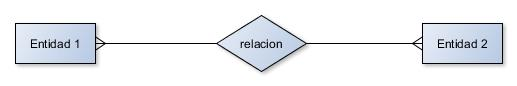
\includegraphics[scale=.75]{./imagenes/ejrelacion.jpg}
    \caption{relacion M:N} 
    \label{fig:graficomn}
  \end{center}
\end{figure}

Una relacion N:1 sera algo de la forma:

\begin{figure}[ht]
  \begin{center}
    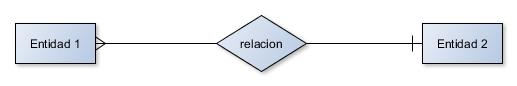
\includegraphics[scale=.75]{./imagenes/ejrelacion2.jpg}
    \caption{relacion N:1} 
    \label{fig:grafico}
  \end{center}
\end{figure}
